% !Mode:: "TeX:UTF-8"
%!TEX program  = xelatex

\documentclass{cumcmthesis}
\usepackage{graphicx}
\usepackage{float}
\usepackage{subfig}
\usepackage{footnote}
% \documentclass[withoutpreface,bwprint]{cumcmthesis} %去掉封面与编号页

\usepackage{url}
\title{基于图论模型的核酸检测点设置位置分析}
\tihao{B}
\baominghao{114514}
\schoolname{天元公学}
\membera{陈铭硕}
\memberb{唐铭泽}
\memberc{尹贝尔}
\supervisor{老师}
\date{\today}
\usepackage{footnote}

\usepackage{graphicx}
\usepackage{float}
\usepackage{subfig}

\begin{document}

\maketitle

\begin{abstract}

\keywords{疫情防控\quad  图论\quad   图的绝对重心\quad  最短路}
\end{abstract}

%目录
\tableofcontents

\newpage
\section{问题重述}

\subsection{问题的提出}

\section{问题分析}

\subsection{总体分析}

一个居民小区通常由一些单元与道路组成。每个单元都有一定数量的人居住,每条道路都有一定的长度。由于是一个小区,任意两个单元可以通过道路相互到达。此外,我们可以
把道路的交叉点等看作没有人居住的单元。核酸检测点可以设在单元里,也可以设在道路上。于是我们可以把居民小区抽象为一张连通无向图,以单元为点,点权为居住人数,边
权为边的长度,把核酸检测点的规划转化成图论问题进行求解。

\subsection{问题一分析}

定义图上两点的花费为两点的最短路径长度乘上起始点的点权。

建立核酸检测点位置要使居民总体方便,那么建立核酸检测点有两种策略:使得每个人到达核酸检测点的路程和最小或到达核酸检测点的最大的路程最短;并且需要考虑建立的位置是否会给居民的正常生活造成影响。

\subsection{问题二分析}

\subsection{问题三分析}

\section{模型假设}



\section{符号说明}
\begin{center}
\begin{savenotes}
\begin{tabular}{cc}
\hline
\makebox[0.3\textwidth][c]{符号}	&  \makebox[0.4\textwidth][c]{意义} \\ \hline
$n$         & 图的点数 \\ \hline
$m$         & 图的边数 \\ \hline
$w_i$	    & 第 $i$ 个点的点权 \\ \hline
$e_i$	    & 第 $i$ 条边的边权 \\ \hline
$u_i$       & 第 $i$ 条边的起点 \\ \hline
$v_i$       & 第 $i$ 条边的终点 \\ \hline
$d_{i,j}$   & 第 $i$ 个点和第 $j$ 个点最短路径长度 \\ \hline
$s_i$       & 第 $i$ 个点的所有人到核酸检测点的距离和 \\ \hline
\end{tabular}
\end{savenotes}
\end{center}

\section{模型建立、求解与分析}

\subsection{问题一}

\subsubsection{方案一}

使得每一个人到达核酸检测点的路程和最小。

假设核酸检测点在边 $(u_k,v_k)$ 上,设其距 $u_k$ 的距离为 $x(x \in [0,e_k])$,那么它距离 $v_k$ 的距离为 $e_k - x$。

对于点 $i$,点 $i$ 上的所有人到核酸检测点的路程和为 $s_i=w_i\cdot\min\left\{d_{u_k,i}+x,d_{v_k,i}+e_k-x\right\}$。我们可以
把 $s_i$ 随 $x$ 的变化表示在平面直角坐标系上。

我们发现当 $x=\frac{d_{v_k,i}+e_k-d_{u_k,i}}{2}$。

显然可以发现图象一定是一条先升再降的折线或者是直线,因此一定是上凸的。由于每个 $s_i$ 关于 $x$ 是上凸的,所以总路程 $\sum_{i=1}^n s_i$ 也是上凸的。
因此 $\sum_{i=1}^n s_i$ 在区间 $[0,e_k]$ 上的最小值一定在 $x=0$ 或 $x=e_k$ 时取到,即核酸检测点一定在某个点上。

以下是算法过程:

\begin{enumerate}
    \item 使用最短路算法求出 $d_{i,j}$;
    \item 枚举每一个点,求出 $\sum_{i=1}^n s_i$,并更新答案。
\end{enumerate}

如果使用堆优化的 Dijkstra 求解最短路,时间复杂度为 $\Theta(n^2\log m)$,若使用 Floyd,时间复杂度为 $\Theta(n^3)$

\subsubsection{方案二}

使得到达核酸检测点的最长的路程最短。

提出一个概念叫 \emph{图的绝对重心},定义为到所有点的距离的最大值最小的点,那我们的核酸检测点应建立在绝对重心上。

接下来考虑如何求解绝对重心。

假设图的绝对重心在边上,枚举每一条边 $(u_k,v_k)$,钦定图的绝对重心 $c$ 在这一条边上,假设其距 $u_k$ 的距离为 $x(0 \le x \le e_k)$,那么它距离 $v_k$ 的距离为 $e_k - x$。

如图绝对重心 $c$ 与一点 $i$ 的关系图:

\begin{figure}[H]
    \centering
    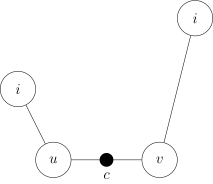
\includegraphics{images/mdst-graph.png}
    \caption{图的绝对中心与一点的位置关系\cite{oiwiki-dmst}}
    \label{fig:mdst-graph}
\end{figure}

那么 $d_{c,i} = \min\left\{d_{u_k, i} + x, d_{v_k,i} + e_k - x\right\}$。

随着 $c$ 从 $u_k$ 到 $v_k$ 的移动 $d_{c,i}$ 的变化如图可以画到一个平面直角坐标系上:

\begin{figure}[H]
	\centering
	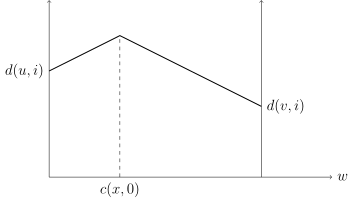
\includegraphics{images/mdst-plot1.png}
	\caption{图的绝对中心变化的影响\cite{oiwiki-dmst}}
	\label{fig:mdst-graph}
\end{figure}

显然可以发现图象会是两条斜率相同的一次函数所构成。

接下来将对于每一个点 $i$ 都画像这样的图象就可以得到:

\begin{figure}[H]
	\centering
	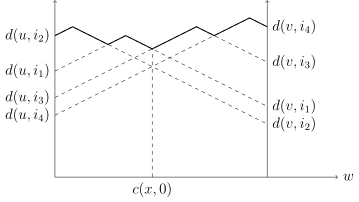
\includegraphics{images/mdst-plot2.png}
	\caption{图的绝对中心变化的影响\cite{oiwiki-dmst}}
	\label{fig:mdst-graph}
\end{figure}

这些折线交点中的最低点,横坐标就是图的绝对中心的位置。

不难发现,出现交点的条件是 $d_{u,i_1} < d_{u,i_2},d_{v,i_1} > d_{v,i_2}$。

对于绝对中心在一个点上,那么就枚举一下那个节点,再用与其距离最远的节点更新一下就行了。

对于每一条边,每一个点都这样做一下就可以了。

总结一下过程:

\begin{enumerate}
    \item 使用最短路算法求出 $d_{i,j}$;
    \item 对于绝对中心在点上更新答案;
    \item 对于绝对中心在边上,枚举每一条边更新答案。
\end{enumerate}

如果使用堆优化的 Dijkstra 求解最短路,时间复杂度为 $\Theta(n^2\log m + nm)$,若使用 Floyd,时间复杂度为 $\Theta(n^3 + nm)$

容易发现,这种实现方式不易推广。



\subsection{问题二}

\subsubsection{方案一}



\subsubsection{方案二}



\section{模型评价}


\bibliographystyle{plain}
\bibliography{ref}
\newpage

%附录
\begin{appendices}


\section{问题一方案一代码}

\begin{lstlisting}[language=cpp]
#include <iostream>
using namespace std;
typedef long long ll;
const ll INF = 1e18;

int N, M;
ll G[510][510], Dist[510][510], Rank[510][510], W[510];

void Center_Point(int &u, int &v, double &x) { //返回值为绝对中心在边 $(u,v)$,与 $u$ 的距离为 $x$
    for (int k = 1; k <= N; k++) {
        for (int i = 1; i <= N; i++) {
            for (int j = 1; j <= N; j++) {
                Dist[i][j] = min(Dist[i][j], Dist[i][k] + Dist[k][j]);
            }
        }
    }

    for (int i = 1; i <= N; i++) {
        for (int j = 1; j <= N; j++) Rank[i][j] = j;
        for (int j = 1; j <= N; j++) {
            for (int k = j + 1; k <= N; k++) {
                if (Dist[i][Rank[i][j]] > Dist[i][Rank[i][k]]) {
                    swap(Dist[i][Rank[i][j]], Dist[i][Rank[i][k]]);
                }
            }
        }
    }

    double Ans = 1e18;

    for (int i = 1; i <= N; i++) {
        for (int j = 1; j <= N; j++) {
            if (i == j || G[i][j] == INF) continue;
            int p = Rank[i][N];
            ll Temp = W[i] * Dist[i][p];
            if (Ans > Temp) {
                Ans = Temp;
                u = i;
                v = j;
                x = 0.00;
            }
            for (int k = N - 1; k >= 1; k--) {
                int t = Rank[i][k];
                if (Dist[j][t] > Dist[j][p]) {
                    Temp = W[i] * (Dist[i][t] + Dist[j][p] + G[i][j]);
                    if (Ans > Temp) {
                        Ans = Temp;
                        u = i;
                        v = j;
                        x = (Dist[j][p] + Dist[i][j] - Dist[i][t]) / 2.00;
                    }
                    p = t;
                }
            }
        }
    }
    return;
}
\end{lstlisting}

\section{问题一方案二代码}

\begin{lstlisting}[language=cpp]
#include <iostream>
using namespace std;
typedef long long ll;
const ll INF = 1e18;

int N, M;
ll G[510][510], Dist[510][510], Rank[510][510], W[510];

int Solve() { // 返回核酸检测点位置
    for (int k = 1; k <= N; k++) {
        for (int i = 1; i <= N; i++) {
            for (int j = 1; j <= N; j++) {
                Dist[i][j] = min(Dist[i][j], Dist[i][k] + Dist[k][j]);
            }
        }
    }

    int ans=0;ll r=INF;
    for(int i = 1; i <= N; i++){
        ll t=0;
        for(int j = 1;j <= N; j++){
            t += Dist[i][j] * W[j];
        }
        if(t<r) ans = i, r = t;
    }

    return ans;
    
    return;
}
\end{lstlisting}

\end{appendices}

\end{document} 